% $Header: /home/vedranm/bitbucket/beamer/solutions/generic-talks/generic-ornate-15min-45min.en.tex,v 90e850259b8b 2007/01/28 20:48:30 tantau $

\documentclass{beamer}

% This file is a solution template for:

% - Giving a talk on some subject.
% - The talk is between 15min and 45min long.
% - Style is ornate.



% Copyright 2004 by Till Tantau <tantau@users.sourceforge.net>.
%
% In principle, this file can be redistributed and/or modified under
% the terms of the GNU Public License, version 2.
%
% However, this file is supposed to be a template to be modified
% for your own needs. For this reason, if you use this file as a
% template and not specifically distribute it as part of a another
% package/program, I grant the extra permission to freely copy and
% modify this file as you see fit and even to delete this copyright
% notice.


\mode<presentation>
{
  \usetheme{Warsaw}
  % or ...

  \setbeamercovered{transparent}
  % or whatever (possibly just delete it)
}

      \newtheorem{proposition}[theorem]{Proposition}
      \theoremstyle{example}
      \newtheorem{game}[theorem]{Game}
      \theoremstyle{definition}
      \newtheorem{question}[theorem]{Question}

\usepackage[english]{babel}
% or whatever

\usepackage[latin1]{inputenc}
% or whatever

\usepackage{times}
\usepackage[T1]{fontenc}
% Or whatever. Note that the encoding and the font should match. If T1
% does not look nice, try deleting the line with the fontenc.


\usepackage{marvosym} % For \Smiley
\usepackage{verbatim} % for \verbatiminput

\usepackage{pgf}
\usepackage{tikz}
\usetikzlibrary{matrix} % for diagrams

\title
{Applications of almost compatible functions for limited information strategies in infinite length games}

\subtitle
{BEST 2015 - San Francisco State University} % (optional)

\author%[Author, Another] % (optional, use only with lots of authors)
{Steven~Clontz~\\http://stevenclontz.com}%\inst{1} \and S.~Another\inst{2}}
% - Use the \inst{?} command only if the authors have different
%   affiliation.

\institute[Auburn, AL] % (optional, but mostly needed)
{
  %\inst{1}%
  Auburn, AL}
  %\and
  %\inst{2}%
  %Department of Theoretical Philosophy\\
  %University of Elsewhere}
% - Use the \inst command only if there are several affiliations.
% - Keep it simple, no one is interested in your street address.

\date[15-06-16] % (optional)
{June 16, 2016}


% If you have a file called "university-logo-filename.xxx", where xxx
% is a graphic format that can be processed by latex or pdflatex,
% resp., then you can add a logo as follows:

 % \pgfdeclareimage[height=1cm]{university-logo}{auburn_logo.png}
 % \logo{\pgfuseimage{university-logo}}



% Delete this, if you do not want the table of contents to pop up at
% the beginning of each subsection:
%\AtBeginSubsection[]
%{
%  \begin{frame}<beamer>{Outline}
%    \tableofcontents[currentsection,currentsubsection]
%  \end{frame}
%}


% If you wish to uncover everything in a step-wise fashion, uncomment
% the following command:

%\beamerdefaultoverlayspecification{<+->}

% Strategy uparrow shortcuts
\newcommand{\win}{\uparrow}
\newcommand{\prewin}{\underset{\text{pre}}{\uparrow}}
\newcommand{\markwin}{\underset{\text{mark}}{\uparrow}}
\newcommand{\tactwin}{\underset{\text{tact}}{\uparrow}}
\newcommand{\kmarkwin}[1]{\underset{#1\text{-mark}}{\uparrow}}
\newcommand{\ktactwin}[1]{\underset{#1\text{-tact}}{\uparrow}}
\newcommand{\codewin}{\underset{\text{code}}{\uparrow}}
\newcommand{\flexmarkwin}{\underset{\text{flexmark}}{\uparrow}}
\newcommand{\semiflexmarkwin}{\underset{\text{semiflexmark}}{\uparrow}}
\newcommand{\limitwin}{\underset{\text{limit}}{\uparrow}}
\newcommand{\notwin}{\not\uparrow}
\newcommand{\notprewin}{\underset{\text{pre}}{\not\uparrow}}
\newcommand{\notmarkwin}{\underset{\text{mark}}{\not\uparrow}}
\newcommand{\nottactwin}{\underset{\text{tact}}{\not\uparrow}}
\newcommand{\notkmarkwin}[1]{\underset{#1\text{-mark}}{\not\uparrow}}
\newcommand{\notktactwin}[1]{\underset{#1\text{-tact}}{\not\uparrow}}
\newcommand{\notcodewin}{\underset{\text{code}}{\not\uparrow}}
\newcommand{\notflexmarkwin}{\underset{\text{flexmark}}{\not\uparrow}}
\newcommand{\notsemiflexmarkwin}{\underset{\text{semiflexmark}}{\uparrow}}
\newcommand{\notlimitwin}{\underset{\text{limit}}{\not\uparrow}}

\newcommand{\oneptcomp}[1]{#1^\star} % deprecated
\newcommand{\oneptlind}[1]{#1^\dagger} % deprecated
\newcommand{\onePtComp}[1]{#1^\star}
\newcommand{\onePtLind}[1]{#1^\dagger}


% Games
\newcommand{\gruConGame}[2]{Gru_{O,P}^{\to}\left({#1},{#2}\right)}
\newcommand{\gruConGameHard}[2]{Gru_{O,P}^{\to,\star}\left({#1},{#2}\right)}
\newcommand{\gruClusGame}[2]{Gru_{O,P}^{\leadsto}\left({#1},{#2}\right)}
\newcommand{\gruClusGameHard}[2]{Gru_{O,P}^{\leadsto,\star}\left({#1},{#2}\right)}

\newcommand{\gruKPGame}[1]{Gru_{K,P}\left({#1}\right)}
\newcommand{\gruKLGame}[1]{Gru_{K,L}\left({#1}\right)}

\newcommand{\cloPFGame}[1]{PtFin_{F,C}\left({#1}\right)}

\newcommand{\menGame}[1]{Men_{C,F}\left({#1}\right)}
\newcommand{\rothGame}[1]{Roth_{C,S}\left({#1}\right)}
\newcommand{\rothAltGame}[1]{Roth_{P,O}\left({#1}\right)}

\newcommand{\barmanDowFanGame}[2]{BD_{B,F}\left({#1},{#2}\right)}

% deprecated, use Scheeper's name instead
\newcommand{\cloFillStrictGame}[1]{Fill^{\cup,\subset}_{C,F}\left({#1}\right)}
\newcommand{\cloFillGame}[1]{Fill^{\cup,\subseteq}_{C,F}\left({#1}\right)}
\newcommand{\cloFillInitialGame}[1]{Fill^{1,\subseteq}_{C,F}\left({#1}\right)}
\newcommand{\cloFillIntGame}[1]{Fill^{\cap}_{C,F}\left({#1}\right)}

\newcommand{\schFillStrictGame}[1]{Sch^{\cup,\subset}_{C,F}\left({#1}\right)}
\newcommand{\schFillGame}[1]{Sch^{\cup,\subseteq}_{C,F}\left({#1}\right)}
\newcommand{\schFillWeakGame}[1]{Sch^{\cup}_{C,F}\left({#1}\right)}
\newcommand{\schFillInitialGame}[1]{Sch^{1,\subseteq}_{C,F}\left({#1}\right)}
\newcommand{\schFillIntGame}[1]{Sch^{\cap}_{C,F}\left({#1}\right)}

\newcommand{\bellUniGame}[1]{Bell_{D,P}^{\textrm{uni}}\left({#1}\right)}
\newcommand{\bellConGame}[1]{Bell_{D,P}^{\rightharpoonup}\left({#1}\right)}
\newcommand{\bellConHardGame}[1]{Bell_{D,P}^{\rightharpoonup,\star}\left({#1}\right)}
\newcommand{\bellAbsConGame}[1]{Bell_{D,P}^{\to}\left({#1}\right)}
\newcommand{\bellAbsConHardGame}[1]{Bell_{D,P}^{\to,\star}\left({#1}\right)}



\newcommand{\SigmaProdR}[1]{\Sigma\mathbb{R}^{#1}}
\newcommand{\SigmaStarProdR}[1]{\Sigma^\star\mathbb{R}^{#1}}
\newcommand{\SigmaProdTwo}[1]{\Sigma2^{#1}}
\newcommand{\sigmaProdTwo}[1]{\sigma2^{#1}}

\newcommand{\concat}{{^\frown}}
\newcommand{\rest}{\restriction}
\newcommand{\offset}{\downharpoonright}

\newcommand{\cl}[1]{\overline{#1}}

\newcommand{\pow}[1]{\mc{P}(#1)}

\newcommand{\<}{\langle}
\renewcommand{\>}{\rangle}

\newcommand{\al}[1]{{#1}^*}

\newcommand{\mc}[1]{\mathcal{#1}}
\newcommand{\mb}[1]{\mathbb{#1}}

\newcommand{\po}{\mathbb{P}}
\newcommand{\pok}{\po_\kappa}

\newcommand{\Lim}{\mathrm{Lim}}
\newcommand{\Suc}{\mathrm{Suc}}

\newcommand{\ds}{\displaystyle}

\newcommand{\st}[2]{st\left(#1,#2\right)}

\newcommand{\alcomp}{\al\parallel}

\newcommand{\rank}{\textrm{rank}}
\newcommand{\dom}{\textrm{dom}}

\renewcommand{\mod}{\,\textrm{mod}}

\newcommand{\zip}{\bowtie}
\newcommand{\ran}[1]{\text{range}(#1)}

\newcommand{\cf}[1]{\textrm{cf}(#1)}

\newcommand{\alcompS}[1]{S(#1)}


\newcommand{\scish}{almost-$\sigma$-(relatively compact)}

\usepackage{mathrsfs}
\newcommand{\pl}[1]{\mathscr{#1}}



\newcommand{\term}{\textit}


\newcommand{\bakergame}[1]{{Bak}_{A,B}(#1)} % deprecated
\newcommand{\bmgame}[1]{{BM}_{E,N}(#1)} % deprecated
\newcommand{\bakerGame}[1]{{Bak}_{A,B}(#1)}
\newcommand{\bmGame}[1]{{BM}_{E,N}(#1)}




\begin{document}
\renewcommand{\pause}{}
\newcommand{\vpause}{\pause\vspace{1em}}

\begin{frame}
  \titlepage
\end{frame}

\section{Motivation}

\subsection{Menger's property and game}

\begin{frame}\small
  \begin{definition}
    A topological space \(X\) is Menger if for every sequence
    \(\<\mc U_0,\mc U_1,\dots\>\)
    of open covers of \(X\) there exists a sequence
    \(\<F_0,F_1,\dots\>\) such that
    \(F_n\) is covered by some finite subcollection of \(\mc U_n\)
    and \(X=\bigcup_{n<\omega}F_n\).
    \begin{figure}
      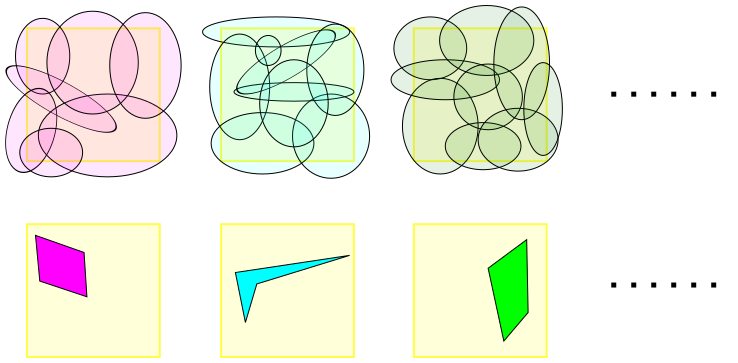
\includegraphics[width=0.6\linewidth]{mengerProperty.pdf}
    \end{figure}
  \end{definition}

  \pause

  \begin{proposition}
    \(X\) is \(\sigma\)-relatively-compact
      \(\Rightarrow\)
    \(X\) is Menger
      \(\Rightarrow\)
    \(X\) is Lindel\"of.
  \end{proposition}
\end{frame}

\begin{frame}
  \begin{game}
    Let \(\menGame{X}\) denote the \term{Menger game} with players
    \(\pl C\), \(\pl F\).

    \begin{figure}
      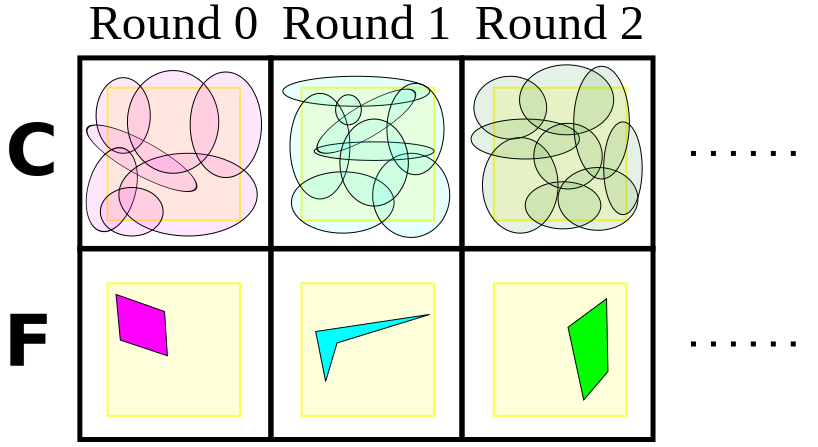
\includegraphics[width=0.6\linewidth]{mengerGame.pdf}
    \end{figure}

    \(\pl F\) wins the game if
    \(X=\bigcup_{n<\omega} F_n\), and \(\pl C\) wins otherwise.
  \end{game}
\end{frame}

\begin{frame}

  \begin{theorem}[Hurewicz 1926 \cite{MR1544773}]
    \(X\) is Menger if and only if \(\pl C \not\win \menGame X\).
  \end{theorem}

  \pause

  \begin{theorem}[Telgarsky 1984 \cite{MR753073}, Scheepers 1995 \cite{MR1273523}]
    Let \(X\) be metrizable. \(\pl F\win\menGame X\) if and only if \(X\) is
    \(\sigma\)-compact.
  \end{theorem}

  \pause

  \begin{theorem}[Fremlin, Miller 1988 \cite{MR954892}]
    There are \(ZFC\) examples of non-\(\sigma\)-compact
    subsets of the real line which are Menger.
  \end{theorem}

\end{frame}

\begin{frame}

  Assume \(\kappa\) is an uncountable cardinal.

  \begin{example}
    Let \(\oneptlind\kappa=\kappa\cup\{\infty\}\), with \(\kappa\)
    discrete and neighborhoods of \(\infty\) being co-countable.
    Then \(\pl F\win\menGame{\oneptlind\kappa}\) but \(\oneptlind\kappa\)
    is not \(\sigma\)-compact.
  \end{example}

\end{frame}

\subsection{Limited information strategies}

\begin{frame}

  \begin{definition}
    A \term{perfect information strategy} uses full information of the
    previous moves of the opponent. (\(\pl A\win G\))
  \end{definition}

  \pause

  \begin{definition}
    A \term{$k$-tactical strategy} only uses the last \(k\)
    previous moves of the opponent. (\(\pl A\ktactwin{k} G\))
  \end{definition}

  \pause

  \begin{definition}
    A \term{$k$-Markov strategy} only uses the last \(k\)
    previous moves of the opponent and the round number.
    (\(\pl A\kmarkwin{k} G\))
  \end{definition}

  \pause

  If omitted, assume \(k=1\).

\end{frame}

\begin{frame}\small
  Considering such strategies allows us to factor out Scheepers's proof
  characterizing \(\sigma\)-compact metrizable spaces with the Menger
  game.

  \pause

  \begin{lemma}
    \(\pl F\markwin\menGame X\) if and only if \(X\) is
    \(\sigma\)-relatively-compact.
  \end{lemma}

  \pause

  \begin{lemma}
    Let \(X\) be second-countable.
    \(\pl F\win\menGame X\) if and only if
    \(\pl F\markwin\menGame X\)
  \end{lemma}

  \pause

  Since metrizable \(+\) Lindel\"of
  \(\Leftrightarrow\) regular \(+\) second countable, we again have
  Telgarsky/Scheepers's result for metrizable spaces.
\end{frame}

\subsection{$k>1$}

\begin{frame}

  \begin{example}
    \(\pl F\win\menGame{\oneptlind\kappa}\), but
    \(\pl F\notmarkwin\menGame{\oneptlind\kappa}\).
  \end{example}

  \pause

  \begin{proposition}
    \(\pl F\kmarkwin{(k+2)}\menGame{X}\) if and only if
    \(\pl F\kmarkwin{2}\menGame{X}\).
  \end{proposition}

  \pause

  \begin{example}
    \(\pl F\kmarkwin{2}\menGame{\oneptlind\omega_1}\)
  \end{example}

  \vpause

  What about for \(\kappa>\omega_1\)? As we'll see, this question
  is not answerable in \(ZFC\).
\end{frame}

\section{Countable-Finite Games and $S(\kappa)$}

\subsection{Scheepers's countable-finite game}

\begin{frame}
  The game \(\menGame{\oneptlind\kappa}\) essentially involves choosing
  countable and finite subsets of \(\kappa\), such as in this game due
  to Scheepers \cite{MR1129143}:

  \begin{game}
    Let \(\schFillStrictGame\kappa\) denote Scheepers's
    \term{strict countable-finite game}
    in which each round \(\pl C\) chooses \(C_n\in[\kappa]^{\leq\omega}\)
    such that \(C_n \supsetneq \bigcup_{i<n}C_i\), followed by \(\pl F\) choosing \(F_n\in[C_n]^{<\omega}\).

    \(\pl F\) wins if \(\bigcup_{n<\omega}F_n=\bigcup_{n<\omega}C_n\),
    and \(\pl C\) wins otherwise.
  \end{game}
\end{frame}

\subsection{Similar countable-finite games}

\begin{frame}
  \(\schFillStrictGame\kappa\) is more restrictive than the Menger game,
  but this is easily remedied.

  \begin{game}
    Let \(\schFillInitialGame\kappa\) denote the
    \term{initial countable-finite game}
    in which each round \(\pl C\) chooses \(C_n\in[\kappa]^{\leq\omega}\)
    such that \(C_n\supseteq \bigcup_{i<n}C_i\),
    followed by \(\pl F\) choosing \(F_n\in[C_n]^{<\omega}\).

    \(\pl F\) wins if \(\bigcup_{n<\omega}F_n\supseteq C_0\),
    and \(\pl C\) wins otherwise.
  \end{game}

  \pause

  \begin{theorem}
    \(\pl F\kmarkwin{k}\schFillInitialGame\kappa\) if and only if
    \(\pl F\kmarkwin{k}\menGame{\oneptlind\kappa}\).
  \end{theorem}
\end{frame}

\begin{frame}
  Perhaps this game is too dissimilar to the original. One may prefer
  to investigate either of these variants as well:

  \pause

  \begin{game}
    Let \(\schFillGame\kappa\) denote the
    \term{nonstrict countable-finite game}
    in which each round \(\pl C\) chooses \(C_n\in[\kappa]^{\leq\omega}\)
    such that \(C_n\supseteq \bigcup_{i<n}C_i\),
    followed by \(\pl F\) choosing \(F_n\in[C_n]^{<\omega}\).

    \(\pl F\) wins if \(\bigcup_{n<\omega}F_n\supseteq \bigcup_{n<\omega}C_n\),
    and \(\pl C\) wins otherwise.
  \end{game}

  \begin{game}
    Let \(\schFillIntGame\kappa\) denote the
    \term{intersection countable-finite game}
    in which each round \(\pl C\) chooses \(C_n\in[\kappa]^{\leq\omega}\),
    followed by \(\pl F\) choosing \(F_n\in[C_n]^{<\omega}\).

    \(\pl F\) wins if \(\bigcup_{n<\omega}F_n\supseteq \bigcap_{n<\omega}C_n\),
    and \(\pl C\) wins otherwise.
  \end{game}
\end{frame}

\begin{frame}[fragile]\small
\begin{theorem}
\begin{tikzpicture}
  \matrix (m) [matrix of nodes,row sep=3em,column sep=1em,minimum width=2em]
  {
    \(\pl F \kmarkwin{k}\menGame{\oneptlind\kappa}\) & &
    \(\pl F \kmarkwin{k}\schFillIntGame\kappa\) \\

    \(\pl F \kmarkwin{k}\schFillInitialGame\kappa\) & &
    \(\pl F \kmarkwin{k}\schFillGame\kappa\) \\

    &
    \(\pl F \ktactwin{k}\schFillStrictGame\kappa\) \\
  };
  \path[>=latex,->]
    (m-1-1) edge (m-2-1)
    (m-1-3) edge (m-2-3)
    (m-3-2) edge (m-2-1)
    (m-3-2) edge (m-2-3);
  \path[>=latex,<->]
    (m-1-1) edge (m-1-3)
    (m-2-1) edge (m-2-3);
\end{tikzpicture}
\end{theorem}
\end{frame}


\section*{}

\begin{frame}[allowframebreaks]
  \tiny
  \bibliographystyle{plain}
  \bibliography{../../bibliography}
\end{frame}

\begin{frame}
  Questions?
\end{frame}

\end{document}


